\documentclass[a5paper,twoside,10pt]{article}
% ******************************************************************************
% ****************************** Custom Margin *********************************

% Add `custommargin' in the document class options to use this section
% Set {innerside margin / outerside margin / topmargin / bottom margin}  and
% other page dimensions
\ifsetCustomMargin
  \RequirePackage[left=37mm,right=30mm,top=35mm,bottom=30mm]{geometry}
  \setFancyHdr % To apply fancy header after geometry package is loaded
\fi

% Add spaces between paragraphs
%\setlength{\parskip}{0.5em}
% Ragged bottom avoids extra whitespaces between paragraphs
\raggedbottom
% To remove the excess top spacing for enumeration, list and description
%\usepackage{enumitem}
%\setlist[enumerate,itemize,description]{topsep=0em}

% *****************************************************************************
% ******************* Fonts (like different typewriter fonts etc.)*************

% Add `customfont' in the document class option to use this section

\ifsetCustomFont
  % Set your custom font here and use `customfont' in options. Leave empty to
  % load computer modern font (default LaTeX font).
  %\RequirePackage{helvet}
  \RequirePackage{lmodern}

  % For use with XeLaTeX
  %  \setmainfont[
  %    Path              = ./libertine/opentype/,
  %    Extension         = .otf,
  %    UprightFont = LinLibertine_R,
  %    BoldFont = LinLibertine_RZ, % Linux Libertine O Regular Semibold
  %    ItalicFont = LinLibertine_RI,
  %    BoldItalicFont = LinLibertine_RZI, % Linux Libertine O Regular Semibold Italic
  %  ]
  %  {libertine}
  %  % load font from system font
  %  \newfontfamily\libertinesystemfont{Linux Libertine O}
\fi

% *****************************************************************************
% **************************** Custom Packages ********************************

% ************************* Algorithms and Pseudocode **************************

%\usepackage{algpseudocode}


% ********************Captions and Hyperreferencing / URL **********************

% Captions: This makes captions of figures use a boldfaced small font.
%\RequirePackage[small,bf]{caption}

\RequirePackage[labelsep=space,tableposition=top]{caption}
\renewcommand{\figurename}{Fig.} %to support older versions of captions.sty


% *************************** Graphics and figures *****************************

%\usepackage{rotating}
%\usepackage{wrapfig}

% Uncomment the following two lines to force Latex to place the figure.
% Use [H] when including graphics. Note 'H' instead of 'h'
%\usepackage{float}
%\restylefloat{figure}

% Subcaption package is also available in the sty folder you can use that by
% uncommenting the following line
% This is for people stuck with older versions of texlive
%\usepackage{sty/caption/subcaption}
\usepackage{subcaption}

% ********************************** Tables ************************************
\usepackage{booktabs} % For professional looking tables
\usepackage{multirow}

%\usepackage{multicol}
%\usepackage{longtable}
%\usepackage{tabularx}


% *********************************** SI Units *********************************
\usepackage{siunitx} % use this package module for SI units
\sisetup{
detect-weight = true,
detect-inline-weight = math
}

% ******************************* Line Spacing *********************************

% Choose linespacing as appropriate. Default is one-half line spacing as per the
% University guidelines

% \doublespacing
% \onehalfspacing
% \singlespacing


% ************************ Formatting / Footnote *******************************

% Don't break enumeration (etc.) across pages in an ugly manner (default 10000)
%\clubpenalty=500
%\widowpenalty=500

%\usepackage[perpage]{footmisc} %Range of footnote options


% *****************************************************************************
% *************************** Bibliography  and References ********************

\usepackage{cleveref} %Referencing without need to explicitly state fig /table

% Add `custombib' in the document class option to use this section
\ifuseCustomBib
   \RequirePackage[square, sort, numbers, authoryear]{natbib} % CustomBib

% If you would like to use biblatex for your reference management, as opposed to the default `natbibpackage` pass the option `custombib` in the document class. Comment out the previous line to make sure you don't load the natbib package. Uncomment the following lines and specify the location of references.bib file

%\RequirePackage[backend=biber, style=numeric-comp, citestyle=numeric, sorting=nty, natbib=true]{biblatex}
%\bibliography{References/references} %Location of references.bib only for biblatex

\fi

% changes the default name `Bibliography` -> `References'; also rewritten in the thesis.tex
\renewcommand{\bibname}{References}


% ******************************************************************************
% ************************* User Defined Commands ******************************
% ******************************************************************************

% *********** To change the name of Table of Contents / LOF and LOT ************

%\renewcommand{\contentsname}{My Table of Contents}
%\renewcommand{\listfigurename}{My List of Figures}
%\renewcommand{\listtablename}{My List of Tables}


% ********************** TOC depth and numbering depth *************************

\setcounter{secnumdepth}{2}
\setcounter{tocdepth}{2}


% ******************************* Nomenclature *********************************

% To change the name of the Nomenclature section, uncomment the following line

%\renewcommand{\nomname}{Symbols}


% ********************************* Appendix ***********************************

% The default value of both \appendixtocname and \appendixpagename is `Appendices'. These names can all be changed via:

%\renewcommand{\appendixtocname}{List of appendices}
%\renewcommand{\appendixname}{Appndx}

% *********************** Configure Draft Mode **********************************

% Uncomment to disable figures in `draft'
%\setkeys{Gin}{draft=true}  % set draft to false to enable figures in `draft'

% These options are active only during the draft mode
% Default text is "Draft"
%\SetDraftText{DRAFT}

% Default Watermark location is top. Location (top/bottom)
%\SetDraftWMPosition{bottom}

% Draft Version - default is v1.0
%\SetDraftVersion{v1.1}

% Draft Text grayscale value (should be between 0-black and 1-white)
% Default value is 0.75
%\SetDraftGrayScale{0.8}


% ******************************** Todo Notes **********************************
%% Uncomment the following lines to have todonotes.

%\ifsetDraft
%	\usepackage[colorinlistoftodos]{todonotes}
%	\newcommand{\mynote}[1]{\todo[author=kks32,size=\small,inline,color=green!40]{#1}}
%\else
%	\newcommand{\mynote}[1]{}
%	\newcommand{\listoftodos}{}
%\fi

% Example todo: \mynote{Hey! I have a note}


\addbibresource{References/references.bib}

\begin{document}

%!TEX root = tezisfuzet.tex

\section*{Tézisfüzet borító angolul}
Lecserélni az angol logós borítóra
\pagebreak

\section*{Description of the topic}

In the past few years, thanks to the experimental and numerical investigations in crystal plasticity, it became clear, that the deformation properties of micron scale crystals essentially differ from what one would expect of bulk samples. In this size scale random rapid discrete events characterise the plastic deformation due to the collective motion of dislocations \cite{Dimiduk1188}, called dislocation avalanches. Therefore, only statistical methods can be used to describe the properties of deformation. The aim of the doctoral thesis is to reveal these almost completely unknown statistical properties by experimental investigation, and to better understand the phenomena by investigating them with computationally simulations. Thanks to the advancement in nanotechnology, more and more micron-scale components are used in the industry, the behaviour of which is essentially affected by the studied phenomena, therefore, the results achieved are expected to have high potential in engineering applications.

\section*{Background and aims}
\markboth{Background and aims}{Numerical models}
\subsection*{Numerical models}

In the first part of my thesis I study the statistical properties of the deformation processes in micron sized samples (e.g. the stress-strain curve, a comparison with a weakest-link model, dislocation-pattern formation) with new models.

Regarding dislocation avalanches, it is known, that they can be modelled not only with computational expensive discrete dislocation dynamics (DDD) simulations\cite{PhysRevLett.112.235501}, but also with larger scale mesoscopic models based on the continuum theory of dislocations\cite{1742-5468-2005-08-P08004}. The appearing free parameters in such models have never been calibrated with larger scale models, although by doing so one would get an effective model, which shows similarity with the lower scale model in the properties attributed to those fitted parameters. The benefit of such model lies in its effectiveness, which means, that using the same computational resource and running time larger systems can be investigated. Such a calibration is possible only if quantities exist, that can be defined and measured on the macroscopic state and properly account for the deformation processes occurring on the microscopic level. Such a model is even more powerful if the similarity of the behaviour is reflected not only in the properties fitted via the parameters but in other respects as well, and if the applicability of the model is wider than the applicability of the lower-scale original model.

\begin{enumerate}
\setcounter{enumi}{0}
\item My aim is to develop a new mesoscopic model based on the continuum theory of dislocations and to calibrate its parameters in such a way, that the behaviour of the model approaches as close as possible the behaviour of the lower scale DDD model in the properties investigated.
\end{enumerate}

Since the first observation of dislocations it is known, that they are almost never distributed homogeneously in the material, but they form various kinds of patterns. This microstructure has an important consequence when it comes to macroscopic behaviour, because they may lead, for instance, to the appearance of persistent slip bands during cyclic deformation leading to fatigue and finally the failure of the material. But dislocation patterns are also responsible for the phenomenon, that deformation response of different micron sized rods (called micropillars) strongly differ from sample to sample. Most of the models describing dislocation patterning use a phenomenological approach. While ones use parameters without explained microscopic origin, others predict behaviours never observed. This is the reason why the model in the work of \citet{PhysRevB.93.214110}, which uses DDD as a basis and set up the continuum model of dislocations meant a significant advancement. In this model each parameter has been defined based on the microstructure and makes it possible to investigate dislocation patterns\cite{PhysRevB.93.214110}. The possibility of pattern formation can be shown by applying linear stability analysis on the model equations, which also connect the macroscopic parameters to the properties of the patterns, e.g. to the size of the characteristic wavelength \cite{PhysRevB.93.214110}. Even though one can hardly state anything apart from their existence on the developed patterns or its robustness, numerical implementations of the mathematical model make it possible to investigate these properties.

\begin{enumerate}
\setcounter{enumi}{1}
\item My aim is to develop a new mesoscopic model based on the continuum theory of dislocations, which is capable of observing and describing dislocation pattern formation beyond the linear stability analysis and makes it possible to investigate the robustness of the patterns evolved.

\end{enumerate}

\subsection*{Experiments}
\markboth{Background and aims}{Experiments}
Most of the experiments in connection with dislocation avalanches consist of preparing the micron sized samples using a focused ion beam in a scanning electron microscope and then move them to another device to perform the nanoindentation test. As the fabrication and the indentation happened in separate devices, one cannot follow in situ the staircase-like structures appearing on the surface of the sample. With a nanoindenter, which fits into the vacuum chamber of a scanning electron microscope with the samples together, one could perform in situ experiments.

Large amount of data can be obtained originating from the structural changes in the samples by detection of the acoustic signals. However, it is challenging to assign the different parallel competing processes to the signals they emit, because most of the signals -- in case of bulk samples -- come from the inner part of the sample, and the change can be observed only on microscopic scale. With an acoustic emission detector, if one can track the compression in site, one can couple the processes with the signals detected. With this technique we could gain a completely new measurement setup making possible to perform new measurements unknown in the literature. 

\begin{enumerate}
\setcounter{enumi}{2}
\item My aim is to develop a nanoindenter, which makes it possible to set up a measurement, where one can in situ follow the deformation of micropillars in a scanning electron microscope, while the acoustic signals emitted by dislocation avalanches are also detected with an attached acoustic emission detector.
\end{enumerate}

With these two methods the size scale available for simulations and experiments are in the same order of magnitude, therefore, the results are directly comparable. This is a unique feature which helps to better understand micron-scale plasticity.

\section*{Methods}
\markboth{Methods}{Numerical models}
\subsection*{Numerical models}
Based on the work of \citet{1742-5468-2005-08-P08004} I developed and implemented a cellular automaton (CA) model. In this model the material consists of small, separated units, which interact via the emerging stresses due to plastic deformation. The model handles the flow stress on cell-level ($\tau_w$) and it is considered as a random variable and calibrated via lower scale, DDD simulations in such a way, that the distribution of the external stress at the first avalanche is the same that one gets for DDD simulations. The expected value of $\tau_w$ and the size of the applied discrete plastic strain on the cells are calibrated via the comparison of the stress-strain curve of the CA model and two other DDD models. Since $\tau_w$ is a probabilistic variable, the plastic response of the system differs from sample to sample, and its time evolution is nondeterministic for one realisation. To compare the desired parameters, therefore, numerous simulations must be evaluated.

The CA model is also applicable to materials with internal disorder that undergo strain softening, if the subsequent fracture is due to strain localisation. To model this behaviour, a softening mechanism was introduced. Disorder in the material is represented by the distribution of $\tau_w$. This internal disorder does not necessarily originate from the inhomogeneous distribution of dislocations, and the material investigated does not even have to be crystalline. It can be metallic glass, metallic foam, or any other material that meets the criteria mentioned in the first sentence of this paragraph.

To investigate dislocation patterns, I developed a third CA model, that contains additional stress terms in the equation of motions. These stress terms are originated from the dislocation correlations described by the continuum theory of dislocations in local density approximation. In such a model random processes still play an important role, which reflects on the one hand, the initial flow stress-distribution, and, on the other hand, the nondeterministic time evolution of the system. Because of these stochastic processes the details of the evolving dislocation patterns differ from sample to sample but by analysing more simulations one can identify the common properties of them. The characteristic wavelength of the pattern can be obtained from the dislocation density of the individual realisations by averaging the patterns in the Fourier space. The robustness of the system can be investigated by varying the strength of the stochastic terms and by applying different rules for the dynamics.

\subsection*{Experiment}
\markboth{Methods}{Experiment}
With commercially available devices, displacement can be measured up to subnanometer precision with capacitive sensors, and objects can be also moved with similar precision with special linear motors. The stress-strain curve of the sample can be expressed with the displacement of the tip of the nanoindenter and the force acting on the tip. To obtain these values, I designed the body of a nanoindenter consisting three main parts as shown in Fig.~1. The displacement of the frame $d$ relative to the stage can be prescribed with a linear motor. The displacement of the tip $e$ relative to the frame is measured with a capacitive sensor. With these data one can express the change in the shape of the sample as $\epsilon = d - e $, and the elongation of the spring as well, which is $e$. From this latter one can calculate the force acting on the tip after measuring the spring constant.

\begin{figure}[htbp!] 
\centering    
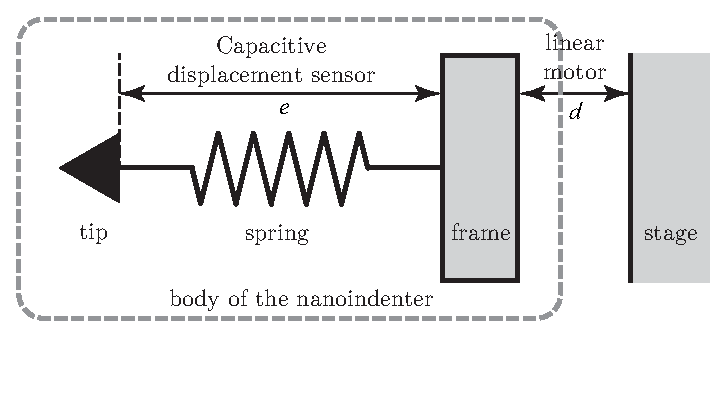
\includegraphics[width=0.9\textwidth]{rugo}
\caption{Schematic structure of the nanoindenter. The unique design of the spring makes it possible, that the tip moves in the deformation axis only. The displacement of the tip relative to the frame is measured by a high precision capacitive displacement sensor. The frame can be moved relative to the stage with subnanometer precision.}
\label{fig:rugo}
\end{figure}

To this end, the nanoindenter body is machined from a single piece of aluminium, where numerous lamellae form the spring. Electric discharge machining provided high enough precision to fabricate such a fine and fragile arrangement. With this setup one can measure the force in the direction of the deformation with \si{\micro\newton} precision, while the tip does not move in the perpendicular directions because of the unique design of the springs. Without this feature the measurement of $d$ with the precision required would become impossible.

Air cannot provide damping in the vacuum chamber, therefore permanent magnets placed below the holder of the tip to achieve the required damping.

\section*{Results}
\markboth{Results}{ }
\begin{enumerate}
\item I showed, that crystalline materials can be resolved into a system of small units, where the size of the units are larger than the correlation length of the dislocations, and such systems can be effectively investigated with cellular automata. By investigating the regime of small deformations, one can calibrate the parameters of the model such a way, that the model shows similar properties to discrete dislocation dynamics simulations. This similarity manifests in the distribution of the external stress of the first avalanches, in its scatter, in its scaling properties with the system size, and in the stress-strain curve. Such a system can be characterised with independent exponents. One of them is the exponent of the power-law-like distribution of the external stress at the first avalanche. While the other one can be obtained by investigating the scatter of the external stress at a given strain value.  \cite{PhysRevB.95.054108}

\item I showed, that materials (i) with internal disorder, which can be considered homogeneous on a larger scale, and (ii) undergo strain softening, and (iii) whose failure is due to strain localisation, can be effectively modelled with cellular automata. I showed that, with increased disorder, even though the onset of plastic regime appears at smaller stresses, a large increase in the applicable highest external stress and in the achievable plastic strain until failure can be observed. \cite{Tuzes2017}

\item It is enough to consider the terms of the equations of motion in the continuum theory of dislocations up to the local density approximation to observe dislocation pattern formation. I showed, that the equations of motion can be solved with a cellular automaton in the presence of stochastic terms, they lead to pattern formation under quite general conditions, and the patterns evolved are in a good agreement with the prediction of the linear stability analysis applied on the original equations of motion.  \cite{PhysRevB.98.054110}

\item I designed and managed the fabrication of a nanoindentation tool, which makes it possible to perform in situ micropillar deformation experiments in a scanning electron microscope, and to which an acoustic emission detector can be attached to associate the processes observed in the electron microscope to the detected acoustic signals. The novel design of the spring in the nanoindenter makes it possible to measure the displacement of the tip relative to the frame with a high accuracy capacitive sensor, and the spring makes it also possible to determine the force acting on the tip. \cite{hegyi}
\end{enumerate}

\section*{Further possibilities}
\begin{itemize}
\item The parameters of the model mentioned in point 2 can be calibrated via lower scale, molecular dynamics models, so that the prediction of the model would have a relevance for real materials.

\item The cellular automata mentioned in point 1 and 3 could be merged together. It is expected that the resulted model would show applicability in the investigation of dislocation avalanches, small plastic deformation regimes and dislocation patterns.

\item The aim of the nanoindentation tool mentioned in point 4 is to facilitate obtaining large data sets on deformations of numerous micropillars. Performing these experiments is an ongoing activity in our research group. It is important to identify the part of the setup which causes the largest noise or difficulty to improve the measurement set-up. For instance, there is a possibility to considerably decrease the mass of the part between the springs and the compression tip making it possible to track the deformation of the micropillars even faster and more precisely.
\end{itemize}


\begin{spacing}{0.9}
\begin{refcontext}[labelprefix=S]
\markboth{Saját publikációim a témában}{ }
\printbibliography[keyword={own_publication}, title={Own publications related to the thesis}, resetnumbers]
\end{refcontext}
\markboth{Irodalomjegyzék}{ }
\printbibliography[notkeyword={own_publication}, title={References},resetnumbers]
\markboth{References}{ }
\end{spacing}

\end{document}


